\documentclass[10pt, conference]{IEEEtran}
\usepackage{graphicx}
\usepackage{grffile}
\usepackage{framed}
\usepackage{amsmath}
\usepackage{booktabs,caption,fixltx2e}
\usepackage[flushleft]{threeparttable}
\usepackage{balance}
\usepackage[dvipsnames]{xcolor}
\usepackage{fancybox}
\usepackage{comment}
\usepackage{pdfpages}
\usepackage{lastpage}
\usepackage{fancyhdr}
\usepackage{multirow}
\usepackage{url}
\pagestyle{fancy}
\renewcommand{\headrulewidth}{0pt}

\newcommand{\todo}[1]{{\color{green}{\textbf{TODO: [#1]}}}}
\newcommand{\emad}[1]{{\color{red}{\textbf{Emad: [#1]}}}}
\newcommand{\ea}{{\em et al.}}
\newcommand{\smallsection}[1]{\vspace{1mm}\noindent {\bf #1}.\hspace{2mm}}
\newcommand{\emphsection}[1]{\vspace{1mm}\noindent \underline{{\em #1}}:\hspace{2mm}}

\newcommand{\revised}[1]{{\color{red}{#1}}}
\newcommand{\conclusionbox}[1]{%
    \vspace{2mm}
  \noindent
    \framebox[0.48\textwidth][c]{%
        \parbox[b]{0.45\textwidth}{%
            {\em #1}
        }
    }
}

\usepackage{array}

\newcolumntype{R}[1]{>{\raggedleft\let\newline\\\arraybackslash\hspace{2pt}}m{#1}}
\cfoot{\thepage\ of \pageref{LastPage}}
% Some very useful LaTeX packages include:
% (uncomment the ones you want to load)

% correct bad hyphenation here
\hyphenation{op-tical net-works semi-conduc-tor}


\begin{document}

\title{Quantifying the Interest of Self-Admitted Technical Debt: A Study using Software Metrics}

% author names and affiliations
% use a multiple column layout for up to two different
% affiliations

%\begin{comment}
\author{\IEEEauthorblockN{Yasutaka Kamei}
\IEEEauthorblockA{Kyushu University, Japan\\
  kamei@ait.kyushu-u.ac.jp\\
}

\and
\IEEEauthorblockN{Everton Maldonado}
\IEEEauthorblockA{Concordia University, Canada\\
e\_silvam@encs.concordia.ca\\
}

\and
\IEEEauthorblockN{Emad Shihab}
\IEEEauthorblockA{Concordia University, Canada\\
	eshihab@encs.concordia.ca\\
}

\and
\IEEEauthorblockN{Naoyasu Ubayashi}
\IEEEauthorblockA{Kyushu University, Japan\\
	ubayashi@ait.kyushu-u.ac.jp\\
}
}
%\end{comment}


\maketitle


\begin{abstract}
Technical debt refers to the phenomena of taking shortcuts to achieve short term gain at the cost of higher maintenance efforts in the future.
Although approaches were developed to detect technical debt through source code comments (i.e., SATD: Self-Admitted Technical Debt), 
the concept of debt, in particular, the cost of debt has not been widely studied.
Therefore, the goal of this paper is to determine ways to measure the ‘interest’ on the debt and use these measures to see how much of the technical debt incurs positive interest, i.e., debt that indeed costs more to pay off in the future. To measure interest, we use the LOC and Fan-In measures. We perform a case study on five open source software projects (Ant, Hadoop, JMeter, Log4j, Tomcat). 
We find that that 10.8\%--31.1\% of technical debt has a positive rate in terms of LOC and 19.3\%--28.1\% of technical debt has it in terms of Fan-In. We should be prioritizing SATD based on its interest, since all SATD is not equal.

\end{abstract}

\begin{IEEEkeywords}
Technical Debt, Software Metrics, Cost, Interest
\end{IEEEkeywords}

\IEEEpeerreviewmaketitle

\section{Introduction}
Technical debt was first coined by Cunningham in 1992 to refer to the phenomena of taking a shortcut to achieve short term development gain at the cost of increased maintenance effort in the future \cite{Cunningham1992WPM}. The technical debt community, organized through the managing technical debt workshop \cite{MTD2016}, has studied many aspects of technical debt, including its detection \cite{Zazworka2013EASE}, impact \cite{Zazworka2011MTD} and the appearance of technical debt in the form of code smells \cite{Fontana2012MTD}. Most recently, we developed an approach to identify technical debt from code comments, referred to as self-admitted technical debt (SATD). SATD refers to the situation where developers know that the current implementation is not optimal and write comments alerting the inadequacy of the solution. 


% What people did and what is the impact of TD. What they found.
In the last few years, an increasing amount of work has focused on SATD. In particular, our prior work focused on the detection of SATD~\cite{Potdar2014ICSME,Maldonado_TSE2017} and the classification of different types of SATD and the development of datasets to enable future studies on SATD~\cite{Maldonado2015MTD}. Other work by Bavota and Russo~\cite{Bavota2016MSR} performed an empirical study of SATD on a large number of Apache projects showed that SATD is prevalent in open source projects, is long lived and is increasing over time. A study by Wehaibi et al.~\cite{Wehaibi2016SANER} examined the impact of SATD on quality and found that SATD does not necessarily relate to more defects, however, it does make the software system more complex. 

%However, very little work focused on interest. Also, why is calculating interest difficult
Although the metaphor of technical debt has been well studied, to the best of our knowledge, the cost of debt/interest has not been extensively studied. Measuring the interest of technical debt is one of the challenges in the field, since it requires for the detection of the technical debt, the tracking of the debt over time and the development of measures to accurately quantify this debt. Given that SATD allows us to know the exact method the technical debt exists in, we are able to perform fine-grained analysis of the code, which enables us to quantify interest of the debt. In this paper, the interest refers to the additional difficulty in repaying the debt.

We investigate the use of code metrics, in particular the well-known Lines of Code (LOC) and Fan-In, to measure interest. We use LOC since it highly correlates with most code complexity metrics and Fan-In\footnote{{\sc Understand} calculates Fan-In as the number of inputs a function uses plus the number of unique subprograms calling the function~\cite{FANIN}.} since it allows us to measure how much a piece of code is depended on by other code. Then, we use the developed measure to determine how much of the SATD incurs positive interest. 
%In a case study on the Apache JMeter project, we find that using LOC, 44.2\% and using Fan-In 42.2\% of the SATD in JMeter incurs positive interest.

This paper is an extended version of our earlier preliminary work~\cite{Kamei2016TDA}. We extend our previous work by:

\begin{itemize}
\item We conduct our case study using the data sets that are collected from five open source software projects.
\item We compare the interest of SATD and non-SATD functions.
\item We examine the activities that lead to the introduction and removal of high-interest SATD.  
\end{itemize}

% Organization of the paper
The rest of the paper is organized as follows; Section \ref{sec:approach} introduces our approach to quantify interest of SATD. Section \ref{sec:results} describes a study using the developed measure and Section \ref{sec:discussion} presents our discussion. Finally, Section \ref{sec:conclusion} draws conclusions and our future work.

%-----------------------------------------------------------------------
\begin{figure*}[!t]
  \begin{center}
  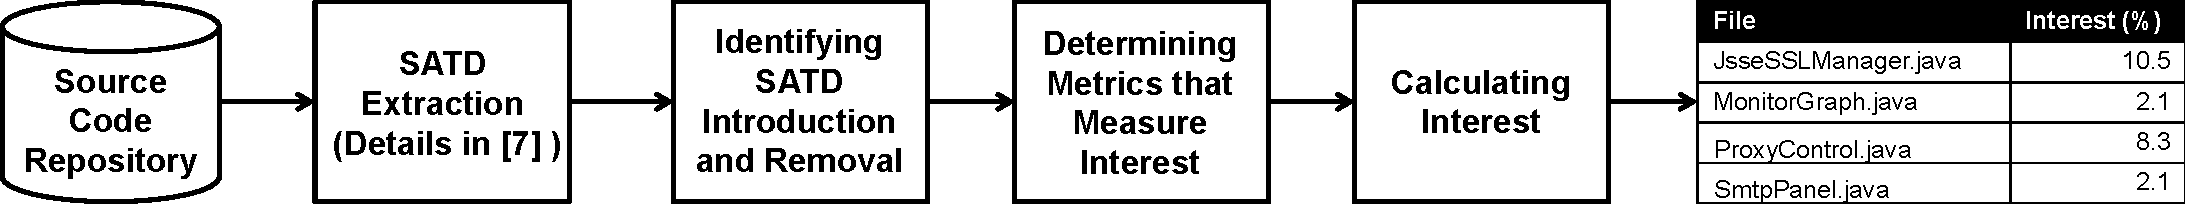
\includegraphics[width=.95\textwidth]{figures/overview}
  \caption{The overview of our approach.}
  \label{fig:overview}
  \end{center}
\end{figure*}
%-----------------------------------------------------------------------

\section{Approach} \label{sec:approach}
In order to conduct our case study, we need to extract SATD from source code comment and identify SATD introduction and removal. Then, we determined metrics that measure interest. Figure \ref{fig:overview} shows the overview of our approach. Below, we describe each step in our approach.

\smallsection{1. SATD Extraction}
In order to measure interest of the TD, our first step is to identify where it exists. Since we focus particularly on SATD, we use code comments found in the source code. We first identify all Java source code files available in the latest version of the project. Then, we analyze the source repository to track all changes done to each file. We take in consideration only the first time that the comment appears on any of the different file versions. This is necessary because the same comment may appear in different versions of the file. 

We parse the source code in order to extract the source code comments. We use an open source library SrcML~\cite{Collard_ICSM2013}, which allows us to parse the source code, and extract the comments and the information related to them such as the line that each comment starts, finishes and the type of the comment (i.e., Javadoc, Line or Block). Then, we apply a series of filters to remove irrelevant comments, e.g., copyright-related comments. Finally, we identify SATD using the NLP classifier presented by Maldonado \ea~\cite{Maldonado_TSE2017}. In this study, we assume that SATD exists in the method where the comment is identified. Details regarding the dataset and the filtering applied can be found in our earlier work~\cite{Maldonado_TSE2017}.

\emphsection{NLP classifier} To train the NLP classifier, we use the manually classified SATD comments dataset provided by Maldonado \ea~\cite{Maldonado_TSE2017}. The dataset contains 62,566 comments extracted from ten open source projects. These comments are classified as SATD comments or as regular comments (i.e., comments without SATD). We use the Stanford NLP Classifier~\cite{Manning2014ACL} to classify SATD comments. The NLP Classifier takes classified data items (comments) as input, and automatically learns features (words) from each datum that are associated with positive or negative numeric votes for each class (SATD or not). Then, we apply the trained NLP classifier to classify the extracted comments from our five studied projects.

% \todo{We need to ask Everton about git commonds to find where it was introduced and removed.
\smallsection{2. Identifying SATD Introduction and Removal}
Since we are interested in measuring the interest, we need to determine the `change' over time in these SATD methods. For each of the SATD comments identified by us, we use several git commands (e.g., {\tt git log -- <PATH\_TO\_FILE>} and {\tt git cat-file <SHA1>:<PATH\_TO\_FILE>}), to trace a comment back to the commit where it was introduced. We perform this task by replaying the history commit-by-commit. Using the same technique, we are also able to detect the removal of SATD. We detect the removal of SATD when we find that the commit is removed or changed. 

\smallsection{3. Determining Metrics that Measure Interest}
Once we are able to determine the SATD comments and their associated methods, we would like to calculate the interest that is incurred over time (i.e., from the introduction of the technical debt to its removal). To do so, we extracted 16 code metrics using the {\sc Understand Tool}~\cite{Understand}. In particular, we selected all method-level complexity and size metrics that Understand is able to provide.

\begin{table*}[tb]
  \caption{Details of studied projects}
  \label{tab:projects}
  \centering

  \begin{tabular}{r|rrrr|rrrr}
  \hline
\textbf{} & \multicolumn{4}{c|}{\textbf{Project details}} & \multicolumn{4}{c}{\textbf{Comments details}} \\ \cline{2-9}
\textbf{Project} & \textbf{\# Java} & \textbf{\# SLOC} & \textbf{\# file} & \textbf{\# contributors} & \textbf{\# comments} & \textbf{\# comments} & \textbf{\# TD} & \textbf{\# unique TD} \\
\textbf{} & \textbf{files} & & \textbf{versions} & & & \textbf{after filtering} & \textbf{ comments} & \textbf{comments} \\
  \hline
Ant        &1,475 & 115,881 & 68,115 & 74 & 1,335,705 & 342,402 & 10,729 &  854  \\
Hadoop     &8,466 & 996,877 & 79,232 &160 & 2,512,673 & 1,172,051 & 18,927 & 1,164 \\
JMeter     &1,181 & 81,307  & 38,091 & 33 & 1,033,390 & 441,780 & 21,356 & 1,260 \\
Log4j      &1,112 & 30,287  & 12,609 & 35 &   248,276 &  61,690 &  1,893 &   135 \\
Tomcat     &3,187 & 297,828 & 46,716 & 32 & 2,336,653 & 1,081,492 & 26,725 & 1,317 \\
  \hline
  \end{tabular}
\end{table*}

\begin{table}[tb]
  \caption{The Percentage of SATD that has Positive, Negative and No Change in Interest \emad{I think we should combine this with table 4 and have it as 1 2-column table}}
  \label{tab:percentage}
  \centering

  \begin{tabular}{cc|rrr}
  \hline
        & & \textbf{Positive} & \textbf{Negative} & \textbf{No Change} \\
  \hline
\multirow{2}{*}{Ant} &  LOC  &  31.1\%  &  12.7\% & 56.2\%\\
                   & Fan-In  &  23.5\%  &  10.8\% & 65.7\%\\
  \hline
\multirow{2}{*}{Hadoop} &  LOC  &  28.4\%  &  11.1\% & 60.5\%\\
                      & Fan-In  &  28.1\%  &  12.5\% & 59.4\%\\
  \hline
\multirow{2}{*}{JMeter} &  LOC  &  25.9\%  &  19.8\% & 54.3\%\\
                      & Fan-In  &  29.2\%  &  9.6\% & 61.2\%\\
  \hline
\multirow{2}{*}{Log4j} &  LOC  &  10.8\%  &  9.2\% & 80.0\%\\
                     & Fan-In  &  19.3\%  &  8.8\% & 71.9\%\\
  \hline
\multirow{2}{*}{Tomcat} &  LOC &  20.6\%  &  12.1\% & 67.3\%\\
                      & Fan-In &  21.5\%  &  9.8\% & 68.7\%\\
  \hline
  \end{tabular}
\end{table}
\begin{table}[tb]
  \caption{Statistics of the SATD that incurs a positive rate}
  \label{tab:statistic}
  \centering

  \begin{tabular}{cc|rrrrr}
  \hline
      &  & \textbf{Min.} & \textbf{1st Qu.} & \textbf{Median} & \textbf{3rd Qu.} & \textbf{Max.} \\
  \hline
\multirow{2}{*}{Ant} &    LOC  & 0.6 &  5.9  &  16.5  &  35.8  &  157.4 \\
                     & Fan-In  & 4.0 & 20.3  &  33.3  &  78.8  &  600.0 \\
  \hline
\multirow{2}{*}{Hadoop} & LOC  & 0.3 &  8.7  &  25.0  &   57.1 &  283.3 \\
                     & Fan-In  & 2.9 & 20.0  &  40.0  &  100.0 &  666.7 \\
  \hline
\multirow{2}{*}{JMeter} & LOC  & 0.5 &  6.7  &  18.2  &   49.5 &  200.0 \\
                     & Fan-In  & 5.9 & 16.7  &  29.7  &   63.5 &  500.0 \\
  \hline
\multirow{2}{*}{Log4j} &  LOC  &  4.7 &  29.5 &  40.7  &   52.7 &   63.4 \\
                     & Fan-In  & 11.1 &  27.6 &  50.0  &  100.0 &  200.0 \\
  \hline
\multirow{2}{*}{Tomcat} & LOC  & 0.4 &  5.3  &  13.6  &   38.7 &  433.3 \\
                     & Fan-In  & 2.0 & 16.7  &  28.6  &   66.7 &  469.2 \\
  \hline
  \end{tabular}
\end{table}


The reasons that we focused on complexity and size metrics are: 1) our intuition tells us that if a piece of code is introduced and then becomes more complex, then that is a good proxy for it being more difficult to deal with in the future, i.e., it incurred interest; and 2) prior work has shown that size metrics are typically highly correlated with complexity metrics, hence, we figured using size metrics (if they are highly correlated with complexity metrics in our case) would be an easier alternative to using complexity metrics.

We measured the Spearman correlation between the complexity and size metrics and found that indeed all metrics except Fan-In are highly correlated with LOC. Therefore, we decided to use the LOC metric as a measure of interest. In addition, since Fan-In is an indicator of how much a method is depended on, we decided to also include the Fan-In metric when calculating interest. The intuition being that if a method is depended on lightly when the SATD is introduced and then has many more dependencies in the future, then dealing with this SATD is much more difficult (since many dependencies may be affected). In the end, we settled on using the two metrics, LOC and Fan-In, as measures of interest.

%To calculate interest, we measure product metrics from two versions detected in Step 2 using {\sc Understand}~\cite{Understand}. We choose all metrics (e.g., LOC and Cyclymatic Complexity) that are available at the method-level in {\sc Understand}.

\smallsection{4. Calculating Interest}
Using our metrics, we consider the relative LOC and Fan-In values between the introduced and removed versions as interest. We calculate the interest per SATD instance. For example, if arbitrary metric values in the introduced and removed versions are 10 and 20 in the method where the SATD exists, the relative size is 100 (i.e, $100* \frac{(20-10)}{10}$). In cases where the SATD is not yet removed, we use the numbers from the latest version of a project. Our assumption here is that if the SATD incurs positive interest, then it will be more difficult to remove in the future, e.g., if the code becomes more complex compared to when the debt was taken, then it will be more difficult to deal with.
% JMeter \emad{shouldn't this be more than just JMeter?}
% that's right. by Yasu

%While the paper tackles the research topic that accelerates a new research direction (i.e., quantifying interest of SATD), it also has the weakness of our current approach. We elaborate on the weakness of our current approach in Section \ref{limitations}.
% \emad{I think we can remove this...what do you think Yasu?}
% I agree. Sounds too weak. by Yasu

\section{Case Study} \label{sec:results}
\smallsection{Motivation}
There exist several previous studies that focused on understanding SATD (e.g., the detection of technical debt~\cite{Potdar2014ICSME,Zazworka2013EASE} and the impact of SATD on software quality~\cite{Wehaibi2016SANER}). However, there are no studies that help in the quantification of SATD interest. Therefore, we would like to know how we can measure interest and if SATD actually incurs positive interest.

\smallsection{Approach}
To calculate interest of SATD, we follow the approach we explained in Section \ref{sec:approach}.
We show the number of SATD, the percentage of the technical debt that has positive interest, and the distribution of interest for technical debt that incurs an positive interest rate.

\smallsection{Datasets}
To conduct our case study, we collect data from six open source software projects (Apache Ant, Hadoop, JMeter, Log4j, Tomcat). Table~\ref{tab:projects} shows details of studied projects. We cloned Git repositories from the selected projects on May 1st 2016. 

\begin{table*}[tb]
  \caption{The Percentage of Software Development Activities when SATD is Introduced/Removed}
  %\emad{I sorted this based on the intro \%}}
  \label{tab:percentage_activities} 
  \centering

  \begin{tabular}{l|r|r|p{2.80in}}
  \hline
       \textbf{Activity} & \textbf{Intro} & \textbf{Removal} & \textbf{Example} \\
  \hline
  New Feature &  36\%  &   8\% &  \textit{HADOOP-9035. Generalize setup of LoginContext (daryn via bobby)} (hadoop -- 86ce5f6) \\
  Refactoring &  30\%  &  54\% &  \textit{moved some code within the acivation area into new methods.} (log4j -- 765875d) \\
  Fix issues  &  18\%  &  23\% &  \textit{fix sizing issue when db is restarted fix JMX domain name fix exception handling} (tomcat -- 525865e). \\
  Testing     &   6\%  &   8\% &  \textit{Correctly define the ROOT context in unit tests} (tomcat -- a2153a3) \\
  Performance &   4\%  &   4\% &  \textit{Do not use Reader and Writer classes for writing response, because [...]} (jmeter -- f88f44b) \textit{HDFS-3726. [...] This isn't critical for correctness but will help reduce log spew on both sides.} (hadoop -- cae8116) \\ 
  Documentation & 2\%  &   4\% &  \textit{Starting the long road of javadoc updates} (jmeter -- 71f6e34), \textit{Better documentation.} (tomcat -- b51444a) \\
     
  Other\      &   4\%  &   0\% & -  \\%\textit{Sometimes my brain just breaks...} (jmeter -- 5c21be0) \\
  \hline
  \end{tabular}
\end{table*}

\smallsection{Results}
Table~\ref{tab:percentage} shows the percentage of the technical debt that has positive interest. The table shows that 10.8\%--31.1\% of technical debt incurs a positive interest rate in terms of LOC and 19.3\%--28.1\% of the SATD has it in terms of Fan-In. We can see that in some cases, there can be negative interest (9.2\%--19.8\% using LOC and 8.8\%--12.5\% using Fan-In), where the SATD method gets smaller or have less Fan-In after the introduction of the SATD. There are also cases where nothing changes in terms of LOC and Fan-In between the SATD introduction and removal. Lastly, it is important to note that there is no large difference between in the amount of positive and no change interest rates using LOC and Fan-In, except for the Log4j project \emad{could we highlight why Log4j behaves this way?}. 

In addition to knowing the amount of SATD that possesses a positive interest rate, we would like to see how high this positive interest is (e.g., is it simply an interest of 1\%, 10\%, 20\%, or higher).
%Next, we would like to know how high is the positive interest rate. This analysis provides us with more insight about the SATD that incurs a positive interest rate.
Table \ref{tab:statistic} shows that the distribution of interest for the SATD that incurs a positive rate \emad{update when we change to a figure?}. We see that the distributions are left-skewed, indicating that the majority of the SATD ranges between 5.3--27.3 and 35.8--100.0 in terms of LOC and Fan-In, respectively. Our findings clearly indicate that there is SATD that incurs a positive interest rate and have different values of interest, which shows that we should be prioritizing SATD based on its interest, i.e., all SATD is not equal.

\conclusionbox{
10.8\%--31.1\% of technical debt incurs a positive rate in terms of LOC and 19.3\%--28.1\% of technical debt incurs it in terms of Fan-In. \emad{should we mention the }}

\section{Discussion} \label{sec:discussion}
Now that we have quantified the amount of SATD that has positive, negative and no interest, along with how high this interest is, we would like to compare the interest of SATD and non-SATD functions. In addition, to shed more light on the activities that lead to high-interest SATD, we also manually examine the activities that lead to the introduction and removal of the highest interest SATD.

\subsection{Comparing the Amount of SATD and Non-SATD}
As shown earlier, we know that approximately between 10-30\% of the SATD functions have positive interest. However, it is not clear if this increase in interest is due to the SATD or is simply due to natural evolution of the code. Therefore, we compare the interest of the SATD and non-SATD functions. 

To ensure that we perform a fair comparison, we do not consider all of the non-SATD functions in the system when comparing interest. Instead, we consider the non-SATD functions from the same files as the SATD functions. Doing so allows for some control of the functions being compared. For each method we follow the same approach as described earlier to measure the interest of SATD functions. In particular, for each file, we compare the LOC and Fan-in of each function (SATD and non-SATD) between the introduction and removal versions.

 
%Generally speaking, software systems are always evolving over time for implementing new functionality and fixing defects~\cite{Robles_IWPSE2005}. Therefore, even if the size of technical debt increases, it is not clear about how the nature of software evaluation affects the interest of technical debt.We would like to compare the impact of software evolution on methods in two groups of SATD v.s. non-SATD.

%\begin{table}[tb]
  \caption{The Percentage of Non-SATD that has Positive, Negative and No Change in Interest}
  \label{tab:percentage_non-SATD} 
  \centering

  \begin{tabular}{cc|p{0.65in}|rrr}
  \hline
        & & \textbf{\# non-SATD instances} & \textbf{Positive} & \textbf{Negative} & \textbf{No Change} \\
  \hline
\multirow{2}{*}{Ant} &  LOC  & \multicolumn{1}{r|}{5,273} &  14.8\%  &  6.8\% & 78.4\%\\
                   & Fan-In  & \multicolumn{1}{r|}{4,924} &  8.6\%  &  5.1\% & 86.3\%\\
  \hline
\multirow{2}{*}{Hadoop} &  LOC  & \multicolumn{1}{r|}{11,247} &  11.0\%  &  4.8\% & 84.2\%\\
                      & Fan-In  & \multicolumn{1}{r|}{10,712} &  17.6\%  &  6.9\% & 75.5\%\\
  \hline
\multirow{2}{*}{JMeter} &  LOC  & \multicolumn{1}{r|}{8,116} &  12.9\%  &  13.1\% & 74.0\%\\
                      & Fan-In  & \multicolumn{1}{r|}{7,566} &  16.4\%  &  6.6\% & 77.0\%\\
  \hline
\multirow{2}{*}{Log4j} &  LOC  & \multicolumn{1}{r|}{1,387} &  11.5\%  &  5.9\% & 82.6\%\\
                     & Fan-In  & \multicolumn{1}{r|}{1,225} &  14.0\%  &  7.3\% & 78.7\%\\
  \hline
\multirow{2}{*}{Tomcat} &  LOC  & \multicolumn{1}{r|}{17,769} &  6.7\%  &  4.6\% & 88.7\%\\
                      & Fan-In  & \multicolumn{1}{r|}{16,487} &  11.0\%  &  5.0\% & 84.0\%\\
  \hline
  \end{tabular}
\end{table}

%\smallsection{Approach}
%We compare the interest of methods between SATD and non-SATD.
%We conduct the following steps:
%\begin{itemize}
%\item [S1:]  We obtain the list of files that include SATD. % from technical_debt_summary.csv
%\item [S2:] We extract methods that do not include SATD in the files that we obtained in S1. % see .method-level.product.csv
%\item [S3:] We measure metrics for the methods that we extracted in S2 at two versions that technical debt is introduced and removed. We only use the methods that can be found at the two versions.
%\item [S4:] We calculate interest using the metrics measured in S3.
%\end{itemize}
% What do we need to do some pre-condition for this analysis?

%\smallsection{Result}

\revised{The right side of Table \ref{tab:percentage}} shows the percentage of non-SATD that has positive, negative, and no change in interest. When we comparing the results of non-SATD with SATD (the left side of Table \ref{tab:percentage}), we find that the positive rate of interest for SATD is larger than non-SATD in all cases except Log4j, according to LOC. \revised{To see whether or not there is a statistical significant difference, we conduct chi-square test to check the positive rate of interest between SATD and non-SATD per project. We use Bonferroni Correction to mitigate the problem of multiple comparisons. The statistical test shows that there is a significant difference between SATD and non-SATD ($p < 0.005$ (= $0.05$ / $10$)) in Ant, Hadoop, JMeter, and Tomcat. 
}
Our finding shows that there is evidence that SATD functions have a higher chance of incurring positive interest compared to normal (or non-SATD) functions.

\emad{can we try to explain why?}. 

% \emad{do you think we can do some sort of statistical test here?}


%We believe that this is one of evidence that SATD is likely to incur positive interest than non-SATD when considering the factor of software evolution.

\subsection{Examining Activities that Lead to the Introduction and Removal of High-interest SATD}

%\smallsection{Motivation}
We have seen that not all SATD incurs positive interest. However, the million dollar question becomes ``what activities lead to the introduction (and removal) of high-interest SATD?''. Answering this question will help us better understand the activities that need to be carefully scrutinized (the case of the introduction of high-interest SATD) and activities that can be encouraged to remove high-interest SATD.


%The interest varies among technical debt. If we can understand the reason why some of technical debt has large interest, we can make use of such insights for future development. Therefore, in this RQ, we would like to manually investigate why some of technical debt has large interest.

%\smallsection{Approach}

To perform our examination, we manually inspected the commits and commit messages of the top 50 highest-interest SATD instances. The sample was based on the interest calculated using Fan-in \emad{why not LOC?}, and included instances from all five projects.

%that introduce and remove technical debt. We choose the top 50 SATD by sorting SATD by Fan-in interest in decreasing order across five projects.

%To highlight the characteristics of technical debt that has large interest, we compare low interest technical debt with high interest technical debt.

\smallsection{Results}
Table \ref{tab:percentage_activities} shows the classification we conducted for top 50 SATD. We find that the largest percentage of high-interest SATD is introduced during the introduction of new features. When developers implement new feature, they tend to not completely finish implementing the new feature in one commit (due to  time pressures, for example). The developers often mention "TODO" or other similar wording to remind them to finish the work later. For example, the commit dbecbe5 in the Hadoop project, which implements MapReduce 2.0, adds SATD "// TODO gross hack". The developer notices that the implementation is not perfect, but conducts such workaround to save his/her development time. Other activities such as refactoring and fixing issues (bugs) are also reasons for the introduction of high-interest SATD. \emad{Yasu, should we add some examples for these two?}


As for the removal of high-interest SATD, refactoring is the top activity, followed by fixing issues (bugs). When developers refactor the code, they tend to also address/remove SATD. For example, the commit c77f96a, which is categorized as refactoring, in the Tomcat project mentions "Drop tomcat-lite module. It never saw a release and has not seen meaningful development for over 4 years."

Overall, our findings indicate that projects should pay attention to SATD introduced during new feature development since such SATD tends to incur high-interest. At the same time, refactoring activities should be encourages, especially since they seem to help remove some of the high-interest SATD.

\emad{Not sure if we should do such analysis for lowest-interest SATD....?}
\subsection{Limitations} \label{limitations}
There are a number of limitations to our study. First, we rely on the NLP classification to determine SATD. This approach is not perfect, achieving an average precision of 0.72 and recall of 0.56~\cite{Maldonado_TSE2017}. Although the precision and recall values are not very high, the NLP technique is considered the state-of-the-art in detecting self-admitted technical debt. Also, the commits were manually classified by the first author. Like any human activity, this process is susceptible to human error. To reduce this bias, the third author validated whether or not the classification results are categorized into an appropriate reason. Lastly, our study is based on open source projects, therefore, our study may not generalize to other open source or commercial projects.

\section{Conclusion} \label{sec:conclusion}
In this paper, we introduced an approach to quantify interest of SATD. Our proposed approach uses software product metrics to lead to measure the interest from software projects.
The results of our case study using five OSS projects show that 10.8\%--31.1\% of technical debt has a positive rate in terms of LOC and 19.3\%--28.1\% of technical debt has it in terms of Fan-In. This finding indicates that that we should be prioritizing SATD based on its interest, i.e., all SATD is not equal.

In the future, we plan to implement a tool that automatically calculate 
the interest of SATD and helps practitioners better understand the impact of SATD on their development process.

\balance
\bibliographystyle{abbrv}
\bibliography{reference}

% that's all folks
\end{document}


